\chapterstart{Kết quả thí nghiệm và so sánh}
\subsection{Mục tiêu và thiết kế đánh giá}
Thực nghiệm tập trung vào hai câu hỏi. Thứ nhất, GLiNER2 có thể trích xuất bảng trên máy cục bộ với chất lượng và thời gian như thế nào khi được cung cấp schema? Thứ hai, khi schema được GPT đề xuất từ một đoạn ngắn, phương án hybrid cho kết quả ra sao so với GPT đọc toàn bài và tạo bảng trực tiếp?

Báo cáo trình bày cấu hình GLiNER2 cuối đã chọn trên validation và đánh giá trên 200 mẫu test. Các phương pháp dùng cùng văn bản và gold, nhưng được chia thành hai điều kiện: schema tham chiếu và tự xác định schema. Đối chiếu GLiNER2 local với GPT trong điều kiện schema tham chiếu đánh giá việc điền dữ kiện; đối chiếu hybrid với GPT trực tiếp đánh giá toàn bộ quá trình từ xác định trường đến tạo bảng. Không quy chênh lệch giữa hai điều kiện chỉ cho năng lực mô hình, vì lượng thông tin đầu vào khác nhau.

\begin{table}[H]
\centering\small
\begin{tabularx}{\linewidth}{@{}p{3.3cm}p{2.1cm}Y@{}}
\toprule\textbf{Phương pháp} & \textbf{Tập đánh giá} & \textbf{Thông tin được cung cấp}\\\midrule
GLiNER2 local & 200 test & Toàn văn và tên bảng/cột từ schema tham chiếu của từng bài; không có tên hàng hoặc giá trị gold.\\
GPT schema tham chiếu & Cùng 200 test & Toàn văn và cùng tên bảng/cột tham chiếu như GLiNER2 local.\\
Hybrid & 200 test & GPT nhận đoạn giữa để đề xuất schema; GLiNER2 nhận schema và toàn văn.\\
GPT trực tiếp & Cùng 200 test & Toàn văn; tự xác định trường và tạo bảng.\\
\bottomrule
\end{tabularx}
\caption{Các phương pháp được báo cáo và điều kiện đầu vào.}
\end{table}

Schema trong hai dòng đầu được dựng từ tên bảng và cột trong gold của chính từng tài liệu. Đây là điều kiện oracle nhằm cô lập bước trích xuất dữ kiện: mô hình không nhận tên hàng hay giá trị gold, nhưng schema không phải thứ hệ thống phải tự suy ra trước khi đọc bài. Vì vậy, kết quả của hai dòng này không đại diện trực tiếp cho một triển khai mà schema chưa được cấu hình từ bên ngoài.

Hai chế độ GPT và hybrid sử dụng kết quả đã lưu; GLiNER2 local được chạy với cấu hình cố định trên đúng 200 ID này. Các đầu ra được chấm theo cùng quy tắc. Các lượt đo diễn ra ở thời điểm khác nhau, nên so sánh dùng cho chất lượng; độ trễ mô tả từng lượt, không dùng để kết luận một tỷ lệ tăng tốc giữa các chiến dịch.

\subsection{Môi trường và cấu hình}
Máy thực nghiệm dùng Apple M1, RAM 16 GiB, macOS ARM64 và Python 3.11.14. GLiNER2 chạy trên CPU, float32, bốn luồng, batch size 1; không yêu cầu GPU trong các phép đo được trình bày. Checkpoint là \code{fastino/gliner2-base-v1}, với revision được cố định:
\begin{center}\code{8437ba583a733d87f56ae902f3b197934eedd58e}\end{center}
 Trọng số không được huấn luyện lại trong dự án.

Schema GLiNER2 giữ tên trường có nghĩa và mô tả gọn; mỗi bảng được thực thi riêng trên toàn bài qua các cửa sổ cần thiết. Ngưỡng trích xuất là 0,5. GPT dùng \code{gpt-5.5}, mức suy luận low, qua Codex CLI 0.154.0-alpha.6.2 và tài khoản ChatGPT; mỗi tác vụ là một phiên mới. Nhánh hybrid không dùng GPT để điền giá trị cuối cùng.

Dữ liệu, schema theo chế độ, lời nhắc và quy tắc chấm được cố định trong từng chiến dịch. Gold chỉ được dùng khi chấm; ở chế độ biết trước schema, mô hình được cung cấp tên bảng/cột nhưng không nhận dữ liệu trong các ô tham chiếu.

\subsection{Chỉ số đánh giá}
\subsubsection{Độ chính xác dữ kiện}
Một dữ kiện là bộ bốn gồm loại bảng, đối tượng, trường và giá trị. Dự đoán chỉ khớp khi các thành phần tương ứng khớp sau chuẩn hóa. Ví dụ, số điểm đúng nhưng gắn nhầm cầu thủ vẫn bị tính là một dữ kiện dự đoán sai và một dữ kiện gold bị thiếu.

Từ tập dự đoán $P_d$ và gold $G_d$ của mỗi tài liệu, chương trình cộng số khớp đúng $TP$, số dự đoán thừa hoặc sai $FP$ và số bị bỏ sót $FN$ trên toàn bộ mẫu. Các chỉ số chính là
\begin{equation}
\mathrm{Precision}=\frac{TP}{TP+FP},\quad
\mathrm{Recall}=\frac{TP}{TP+FN},\quad
F_1=\frac{2TP}{2TP+FP+FN}.
\end{equation}
Đây là fact micro F1, không phải tỷ lệ tài liệu hoàn toàn đúng. Dữ kiện trùng không được tính thêm điểm; null khác 0; các trường lạ vẫn nằm trong dự đoán. Tên bảng, trường và giá trị được chuẩn hóa bằng quy tắc cố định cho các phương pháp.

Mọi mẫu đã thử đều nằm trong điểm tổng, kể cả đầu ra rỗng hoặc lỗi thực thi. Kết quả hợp lệ về cấu trúc chỉ xác nhận chương trình có thể đọc và kiểm tra đầu ra, không xác nhận dữ kiện đúng. Ngoài F1, báo cáo dùng độ bao phủ schema để xác định phần dữ kiện gold thuộc các trường được GPT đề xuất.

\subsubsection{Thời gian và phạm vi đo token}
Độ trễ toàn tác vụ được đo từ lúc chuẩn bị đầu vào đến lúc có bảng cuối hoặc trạng thái lỗi. Với hybrid, thời gian bao gồm GPT tạo schema, GLiNER2 xử lý toàn văn, ghép kết quả và hậu xử lý. Tải trọng số, làm nóng mô hình, chấm điểm và dựng báo cáo không nằm trong thời gian xử lý từng bài.

Thực nghiệm không thống kê token hoặc quy đổi tiền. Vì vậy, nhận định về tiết kiệm token được giới hạn ở thiết kế: GLiNER2 local không gọi dịch vụ LLM để trích xuất; hybrid thu hẹp phần văn bản gửi GPT và chỉ yêu cầu schema thay vì bảng dữ liệu đầy đủ. Chưa có tỷ lệ tiết kiệm token hay chi phí được xác nhận bằng số đo.

\subsection{So sánh trong điều kiện schema tham chiếu trên 200 mẫu test}
Cấu hình GLiNER2 local được giữ nguyên sau khi chọn trên validation và hoàn tất 200/200 mẫu test, với 200/200 đầu ra hợp lệ. Với 6156 dữ kiện gold, mô hình trích khớp 2551 dữ kiện, tạo 2751 dự đoán thừa hoặc sai và bỏ sót 3605 dữ kiện. GLiNER2 và GPT đều nhận cùng tên bảng/trường lấy từ gold của từng bài, nhưng không nhận tên hàng hoặc giá trị gold.

\begin{table}[H]
\centering
\begin{tabularx}{\linewidth}{@{}Yrr@{}}
\toprule
\textbf{Chỉ số} & \textbf{GLiNER2 local} & \textbf{GPT schema tham chiếu} \\\midrule
Precision & 48,11\% & 72,16\% \\
Recall & 41,44\% & 65,51\% \\
Fact micro F1 & \textbf{44,53\%} & \textbf{68,68\%} \\
TP / FP / FN & 2551 / 2751 / 3605 & 4033 / 1556 / 2123 \\
Đầu ra hợp lệ & 200/200 & 200/200 \\
\bottomrule
\end{tabularx}

\caption{So sánh GLiNER2 local và GPT trong điều kiện oracle schema tham chiếu trên cùng 200 mẫu test.}
\label{tab:local}
\end{table}

GLiNER2 local đạt F1 44,53\%, thấp hơn 24,15 điểm phần trăm so với GPT trong điều kiện schema tham chiếu (68,68\%). Khoảng tin cậy 95\% của chênh F1 local trừ GPT là [-28,99; -19,21] điểm phần trăm, tính bằng bootstrap ghép cặp theo tài liệu, 2000 lần, seed 2026. Phép so sánh này phản ánh chất lượng điền dữ kiện khi hai phương pháp được cung cấp cùng schema oracle.

Độ trễ local trung bình là 3,620 giây/bài; median 2,592 giây và P95 9,165 giây. Tổng cộng có 636 lượt forward, xử lý đủ toàn văn cho từng bảng. Tải trọng số và làm nóng mô hình được loại khỏi thời gian từng bài. Toàn bộ lượt local không gọi GPT; kết quả xác nhận khả năng chạy phần trích xuất trên CPU của máy cá nhân.

Recall 41,44\% cho thấy vẫn còn nhiều dữ kiện bị bỏ sót. Lợi ích local nằm ở khả năng giữ văn bản tại máy và không dùng token dịch vụ LLM cho bước trích xuất; kết quả chưa cho thấy chất lượng tương đương GPT trong điều kiện cùng schema oracle. Trong triển khai, schema phải được người dùng/cấu hình cung cấp hoặc được một bước riêng đề xuất, như nhánh hybrid. Do đó, lựa chọn chế độ cần cân nhắc yêu cầu về chất lượng, dữ liệu nội bộ và tài nguyên triển khai.

\subsection{So sánh hybrid với GPT trực tiếp trên 200 mẫu test}
Hybrid hoàn tất 200/200 tác vụ. Kết quả GPT trực tiếp đã lưu cũng bao phủ cùng 200 mẫu, trong đó có một timeout được tính như dự đoán rỗng trong điểm chính. Bảng~\ref{tab:hybrid} trình bày kết quả theo cùng bộ chấm.

\begin{table}[H]
\centering
\begin{tabularx}{\linewidth}{@{}Yrr@{}}
\toprule
\textbf{Chỉ số} & \textbf{Hybrid} & \textbf{GPT trực tiếp} \\\midrule
Precision & 46,03\% & 8,13\% \\
Recall & 17,59\% & 10,79\% \\
Fact micro F1 & \textbf{25,46\%} & \textbf{9,27\%} \\
TP / FP / FN & 1083 / 1270 / 5073 & 664 / 7501 / 5492 \\
Đầu ra hợp lệ & 200/200 & 199/200 \\
\bottomrule
\end{tabularx}

\caption{So sánh chất lượng hybrid và GPT trực tiếp trên cùng 200 mẫu test. Baseline GPT trực tiếp dùng đầu ra đã lưu.}
\label{tab:hybrid}
\end{table}

Hybrid đạt F1 25,46\%, cao hơn 16,18 điểm phần trăm so với F1 9,27\% của GPT trực tiếp. Khoảng tin cậy 95\% cho chênh F1 là [11,89; 20,18] điểm phần trăm, tính bằng bootstrap ghép cặp theo tài liệu, 2000 lần, seed 2026. Khoảng này mô tả biến thiên theo mẫu tài liệu; không bao quát mọi thay đổi của dịch vụ hoặc mọi lần gọi GPT khác.

\begin{figure}[H]
\centering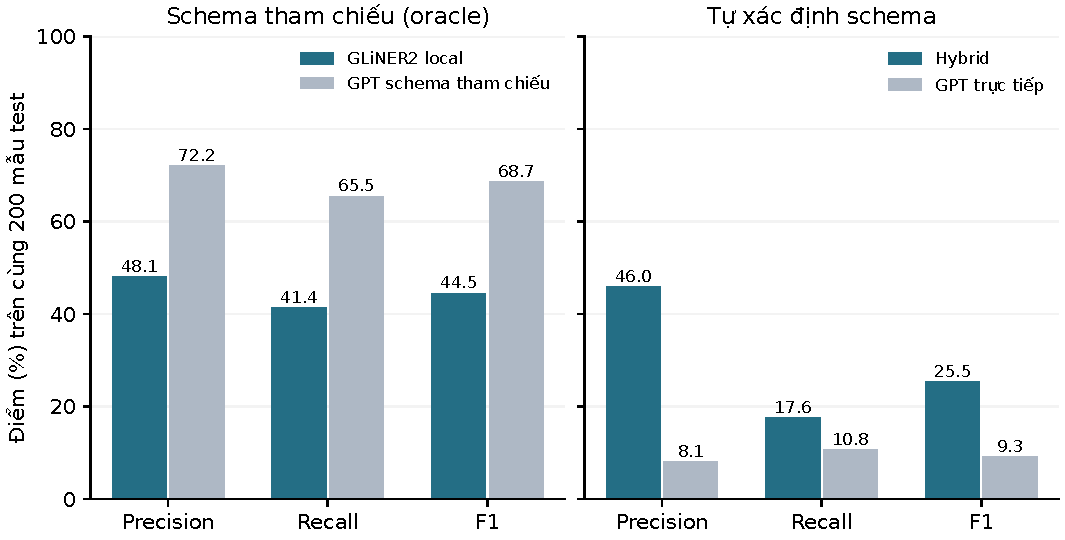
\includegraphics[width=.96\linewidth]{figures/final_comparison.pdf}
\caption{Precision, recall và fact micro F1 trên cùng 200 test, chia theo điều kiện schema tham chiếu và tự xác định schema. Hai chế độ GPT dùng kết quả đã lưu.}
\end{figure}

Cả precision và recall của hybrid đều cao hơn baseline đã lưu trong phép so sánh này. Tuy nhiên, điểm số là mức khớp của toàn bộ pipeline với gold: cách đặt tên bảng/trường, chuẩn hóa giá trị và liên kết định danh đều ảnh hưởng. Một tên gần nghĩa nhưng chưa có trong alias cố định có thể tạo FP/FN. Do đó, kết quả không đồng nghĩa GLiNER2 luôn có khả năng đọc hiểu cao hơn GPT hoặc mọi hệ thống hybrid đều sẽ tốt hơn cách tạo bảng trực tiếp.

\subsection{Độ trễ và trạng thái đầu ra của hybrid}
Hybrid có 200/200 schema hợp lệ, 187 schema chứa thuộc tính, 196 trạng thái success và bốn đầu ra trích xuất rỗng. Không có retry bên ngoài trong lượt đo. Schema không có thuộc tính vẫn có thể tạo hàng chỉ chứa định danh; vì vậy số schema có thuộc tính và số bảng rỗng không phải hai số đếm tương đương.

\begin{table}[H]
\centering
\begin{tabularx}{\linewidth}{@{}Yr@{}}
\toprule
\textbf{Chỉ số} & \textbf{Giây/bài} \\\midrule
Mean e2e & 12,020 \\
Median e2e & 11,552 \\
P95 e2e & 18,126 \\
Mean bước GPT tạo schema & 10,696 \\
Mean bước GLiNER2 & 1,310 \\
\bottomrule
\end{tabularx}

\caption{Độ trễ hybrid trên 200 mẫu; gồm GPT tạo schema và toàn bộ bước GLiNER2 cục bộ.}
\end{table}

Phần lớn độ trễ hybrid nằm ở yêu cầu GPT tạo schema; bước GLiNER2 trung bình khoảng 1,310 giây/bài. Tổng cộng GLiNER2 thực hiện 339 lượt forward để xử lý các bảng và cửa sổ văn bản cần thiết. Việc dùng mô hình cục bộ cho bước điền bảng không loại bỏ độ trễ mạng của bước tạo schema trong hybrid.

Mean 3,620 giây của GLiNER2 local và mean 12,020 giây của hybrid đều được đo trên cùng 200 mẫu test, nhưng ở hai chiến dịch và hai điều kiện schema khác nhau. Các số này mô tả độ trễ từng lượt; không tính tỷ số tăng tốc so với GPT hoặc giữa local và hybrid như một phép đo đồng thời có kiểm soát.

\subsection{Độ bao phủ schema và khác biệt giữa các bảng}
Trong 6156 dữ kiện gold của test, 2395 dữ kiện thuộc các cặp bảng--trường được schema GPT đề xuất, tương ứng 38,91\%. Có 3761 dữ kiện thuộc trường chưa được đề xuất khớp. Trong phần có trường, 1083 dữ kiện được trích khớp và 1312 dữ kiện còn chưa khớp.

\begin{figure}[H]
\centering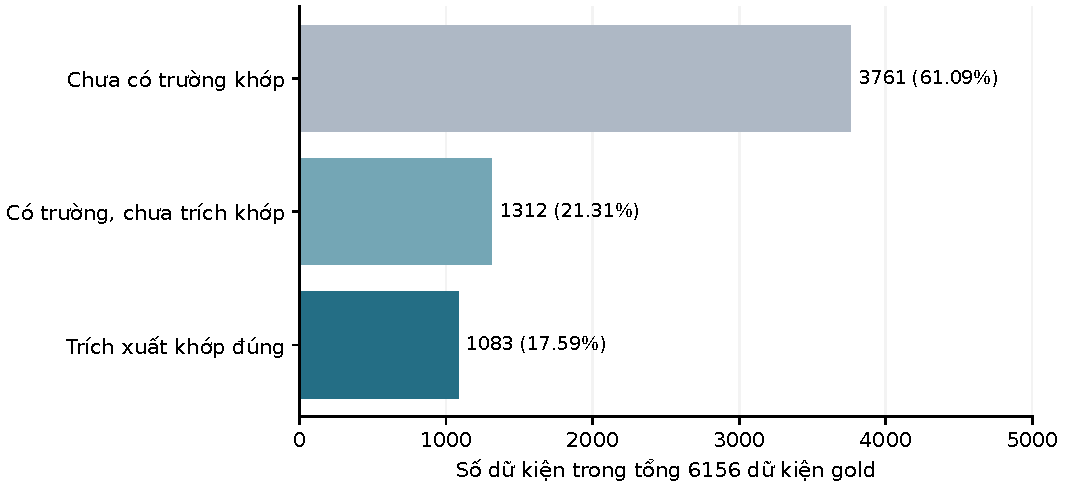
\includegraphics[width=.92\linewidth]{figures/schema_coverage.pdf}
\caption{Phân rã dữ kiện gold theo schema được đề xuất và kết quả trích xuất của hybrid.}
\end{figure}

Phân rã cho thấy hiệu quả hybrid phụ thuộc cả hai giai đoạn: chọn đúng bộ trường và điền đúng các giá trị. Tỷ lệ chưa có trường khớp cũng gồm ảnh hưởng của tên trường chưa có alias, nên không thể quy toàn bộ cho việc đoạn GPT đọc quá ngắn. Việc kiểm tra định dạng schema đạt 100\% chưa giải quyết được các vấn đề ngữ nghĩa này.

\begin{table}[H]
\centering\small\setlength{\tabcolsep}{4pt}
\begin{tabularx}{\linewidth}{@{}Yrrrrrrr@{}}
\toprule
\textbf{Bảng} & \textbf{Gold} & \textbf{TP} & \textbf{FP} & \textbf{FN} & \textbf{P (\%)} & \textbf{R (\%)} & \textbf{F1 (\%)} \\\midrule
Cầu thủ & 4839 & 1069 & 1126 & 3770 & 48,70 & 22,09 & 30,40 \\
Đội & 1317 & 14 & 106 & 1303 & 11,67 & 1,06 & 1,95 \\
\bottomrule
\end{tabularx}

\caption{Kết quả hybrid theo bảng cầu thủ và bảng đội trên 200 test.}
\end{table}

Bảng cầu thủ có 1069 dữ kiện đúng, F1 30,40\%; bảng đội chỉ có 14 dữ kiện đúng, F1 1,95\%. Điểm tổng vì vậy chưa đại diện cho chất lượng đồng đều giữa các loại bản ghi. Macro fact F1 của hybrid là 20,72\%, còn tỷ lệ tài liệu khớp hoàn toàn cả dữ kiện, trường và định danh là 0\%. Các kết quả này cho thấy vẫn cần người kiểm tra khi yêu cầu bảng đầy đủ và chính xác.

\subsection{Ý nghĩa kết quả và phạm vi áp dụng}
Kết quả local chứng minh phần trích xuất của chương trình có thể thực hiện trên CPU với thời gian đo được, phù hợp với định hướng giữ nội dung tài liệu trong môi trường nội bộ và không dùng token dịch vụ LLM cho bước này. Khi bộ trường đã được xác định rõ, đây là chế độ đáp ứng trực tiếp nhất mục tiêu xử lý hoàn toàn cục bộ.

Hybrid bổ sung khả năng đề xuất schema theo nội dung, giúp phần trích xuất không bị cố định vào một tập cột duy nhất. Trên RotoWire, cách chia vai trò này cho điểm khớp dữ kiện cao hơn GPT trực tiếp trong đối chiếu đã thực hiện. Đổi lại, đoạn văn bản dùng tạo schema vẫn được gửi tới GPT và có thể mang thông tin nội bộ; lợi ích của hybrid là giảm phạm vi dữ liệu gửi đi, không phải loại bỏ hoàn toàn việc chia sẻ dữ liệu với dịch vụ ngoài.

Khả năng dùng cho nhiều loại văn bản nằm ở cơ chế schema động và tầng trích xuất có thể tái sử dụng. Để xác nhận cho một miền mới, cần dữ liệu và nhãn của miền đó, mô tả schema phù hợp và đánh giá độc lập. Các kết quả hiện tại chỉ áp dụng cho tiếng Anh trong miền bóng rổ, một checkpoint và một mức suy luận GPT.

Ngoài ra, tập test này đã được sử dụng trong quá trình nghiên cứu trước khi đánh giá cấu hình cuối; chưa phải một tập xác nhận hoàn toàn mới. Dữ liệu cũng chưa được tách sạch theo trận và gold có thể còn thiếu hoặc sai nhãn. Vì vậy, hướng kiểm chứng tiếp theo là đánh giá trên dữ liệu chưa quan sát, tách theo sự kiện và mở rộng miền, đồng thời đo token thực nếu cần công bố mức tiết kiệm định lượng.

\subsection{Kết luận}
Dự án xây dựng phương án trích xuất bảng dựa trên GLiNER2 chạy cục bộ và mở rộng bằng GPT tạo schema từ đoạn ngắn. Trong điều kiện oracle schema tham chiếu, cấu hình local đạt F1 44,53\% trên 200 test, với độ trễ trung bình 3,620 giây/bài; GPT nhận cùng schema đạt F1 68,68\%. Hybrid đạt F1 25,46\% trên 200 test, so với 9,27\% của baseline GPT trực tiếp đã lưu, với mean e2e 12,020 giây/bài.

Giá trị của thiết kế là đưa bước đọc toàn văn và điền dữ kiện về máy cục bộ, đồng thời cho phép thay schema theo nội dung khi cần. Lợi ích về giữ dữ liệu tại chỗ đạt đầy đủ nhất ở chế độ không gọi GPT; lợi ích về giảm token dịch vụ trong hybrid mới được phân tích ở mức cơ chế, chưa được đo định lượng. Khả năng mở rộng đa miền là hướng sử dụng cần kiểm chứng thêm, còn chất lượng đầu ra hiện tại vẫn phụ thuộc độ bao phủ trường và liên kết đúng đối tượng--giá trị.
